We shall see later in class that the linear operator 
\[ L u = -{d^2 \over dx^2} u\]
acting on the vector space $C_D^2[0,1] = \{ u\in C^2[0,1]: u(0)=u(1)=0\}$
has eigenvalues
        \[ \lambda_k(L) = k^2\pi^2, \qquad k = 1, 2, \ldots \]
with corresponding eigenvectors
        \[  v_k(x) = \sin(k\pi x), \qquad k = 1, 2, \ldots.\]
For this problem, we wish to see how well the eigenvalues of this operator
are approximated by the eigenvalues of our matrix
\[ \BA_N = {1\over h^2} \left[\begin{array}{rrrrr}
               2 & -1 \\[0.25em]
              -1 &  2 & -1 \\
                 & -1  &  2 & \ddots \\
                 & & \ddots & \ddots & -1 \\[0.25em]
                 & & & -1 &  2
               \end{array}\right]\in R^{N\times N},\]
where $h=1/(N+1)$ and unspecified entries are zero.

\begin{enumerate}
\item Use the \verb|eig| command in MATLAB to compute the eigenvalues 
      of this matrix for $N=64$.\\ 
      Produce a careful \verb|semilogy| plot showing, on the horizontal
      axis, the index $k$ for $k=1,\ldots N$ and, on the vertical axis,
      the error between the eigenvalues of $\BA_N$ 
      and the exact eigenvalues $\lambda_k(L) = k^2\pi^2$ for the operator $L$.
      Which eigenvalues of $L$ are most accurately approximated?

\item Now create a \verb|loglog| plot showing how the error in the 
      smallest four eigenvalues changes as $N=8$, 16, 32, 64, 128.
      On the horizontal axis you should have $N$, and on the vertical
      axis you should have the error, i.e., $|\lambda_k(\BA_N) - \lambda_k(L)|$.
      There should be one curve each for $k=1, 2, 3, 4$.

\item Comment (qualitatively) on how well the \emph{eigenvectors} of $\BA_N$ 
      approximate those of $L$ for small values of $k$ and $N=64$.  
      You can compute eigenvalues in MATLAB using \verb|[V,D] = eig(A)|.\\
      (Spare a tree: please \emph{do not} print out all the entries of the matrix
       of eigenvectors!)
\end{enumerate}

%%%%%%%%%%%%%%%%%%%%%%%%%%%%%%%%%%%%%%%%%%%%%%%%%%%%%%%%%%%%%%%%%%%%%%%%%%%%%%%%

\ifthenelse{\boolean{showsols}}{\begin{solution}
Code for this problem is included at the end of the solution.
\begin{enumerate}
\item The following plot shows that the \emph{smallest eigenvalues} are most
      accurately approximated.  The larger eigenvalues have quite large errors.

       \begin{center} 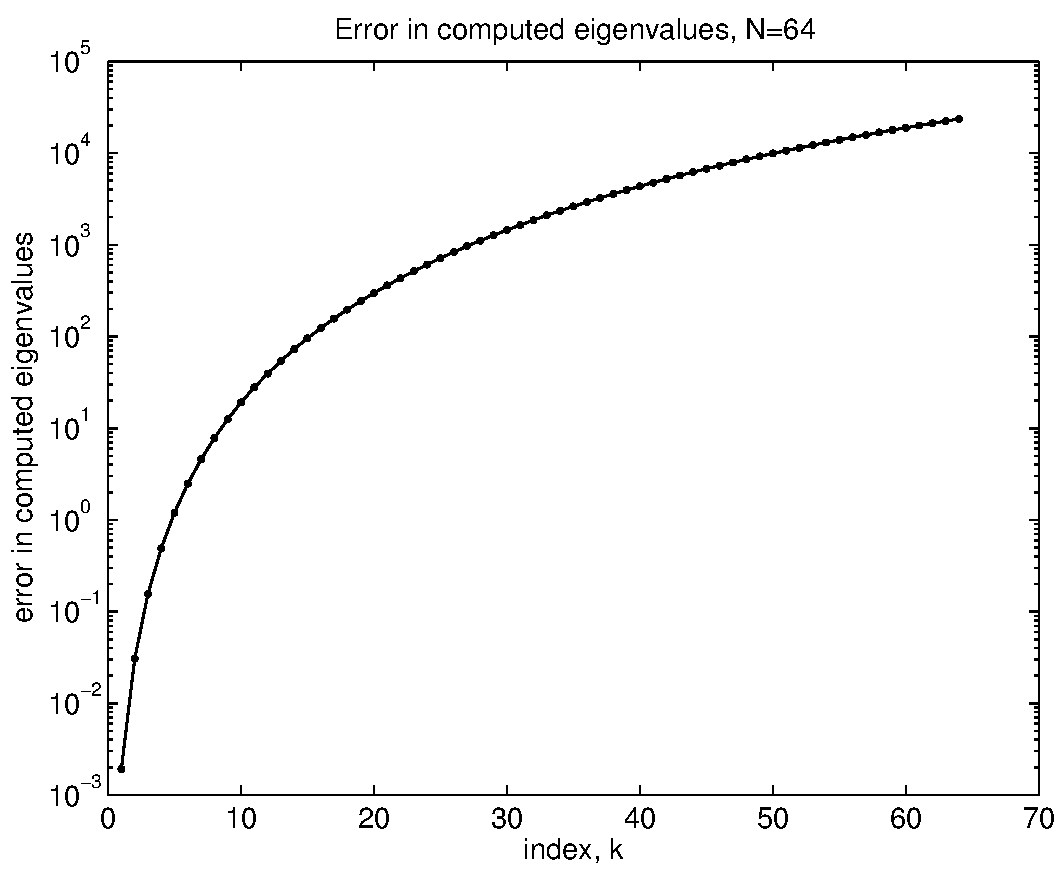
\includegraphics[scale=0.45]{lapeig_a} \end{center}
   
\item The following plot shows a steady decrease in the error of the
      first four eigenvalues as $N$ is increased.  (Here we include 
      extra values of $N$ to emphasize the trend.)  It turns out that
      the error decreases like $1/N^2$, which means that as we double
      $N$, we decrease the error by a factor of $1/4$.
       \begin{center} 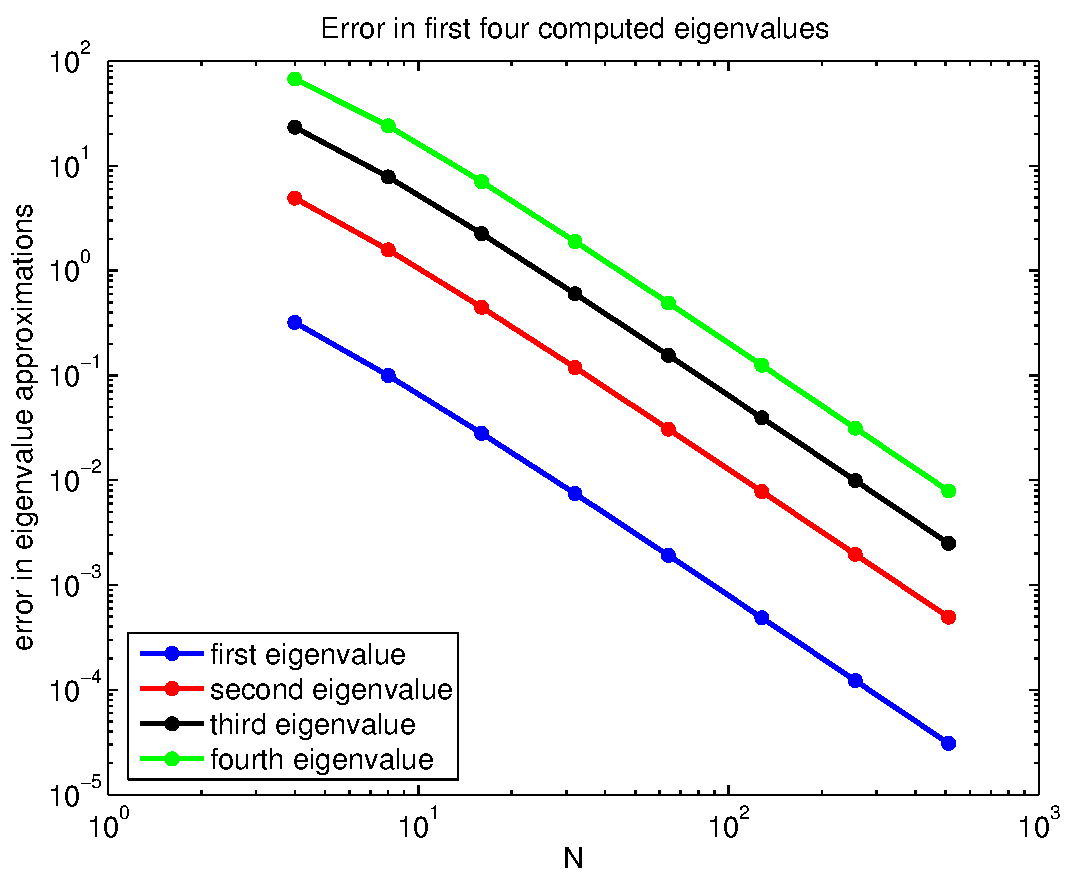
\includegraphics[scale=0.5]{lapeig_b} \end{center}

\item {[\textbf{GRADERS}: Please mark this part of the problem leniently;
       there will probably be considerable confusion over the scaling of 
       the eigenvectors.  Give full marks provided there is evidence
       that the eigenvectors were computed and they were given some modest
       amount of thought.]}

      Recall that if $\Bv$ is an eigenvector of $\BA$ associated with eigenvalue
      $\lambda$, then $\alpha\Bv$ is also an eigenvector associated with $\lambda$
      for any $\alpha\ne 0$.  This scaling is key to comparing the eigenvectors output
      by MATLAB to the true eigenvectors.  Here we choose to scale an $N$-length
      eigenvector $\Bv_k$ such that its first component exactly matches the 
      desired value $\sin(k\pi x)$ at the grid point $x_1=h$.  This scaling is
      accomplished through the line of code
      \texttt{k = vk*sin(k*pi*x(1))/vk(1);}.
      We can then judge the accuracy of the computed eigenvector by comparing
      it to the true eigenfunction at grid points $x_2, \ldots, x_N$.

      The plots on the next page compare the true eigenfunctions with the computed
      eigenvectors for $N=64$ and $k = 1,2, 3, 4, 8, 16, 32, 64$.
      For the smaller values of $k$, it is difficult to see any 
      discrepancy between the true and computed eigenfunctions,
      yet the numerical method does a poor job approximating 
      \emph{high frequency eigenfunctions}---eigenfunctions with
      many oscillations---because there are insufficiently many grid points
      to represent such functions.

      \newpage \vspace*{-5em}
       \begin{center}
         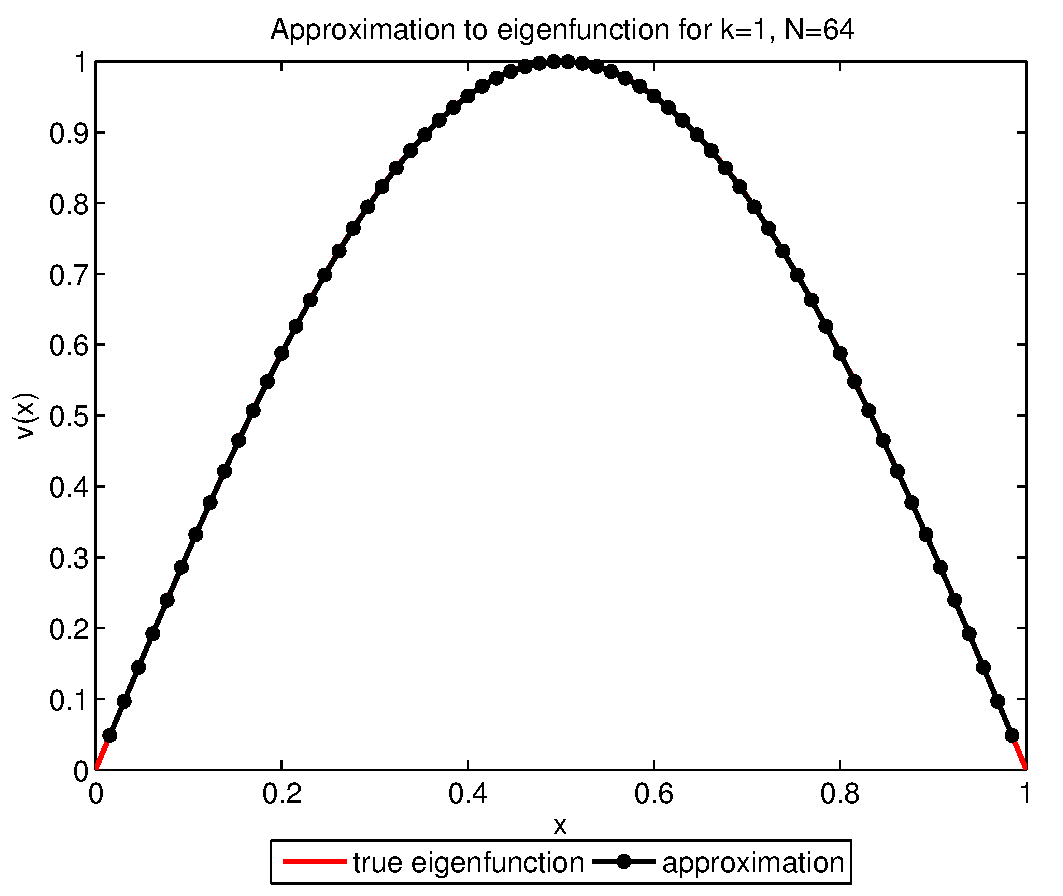
\includegraphics[scale=0.38]{lapeig_c1}\quad
         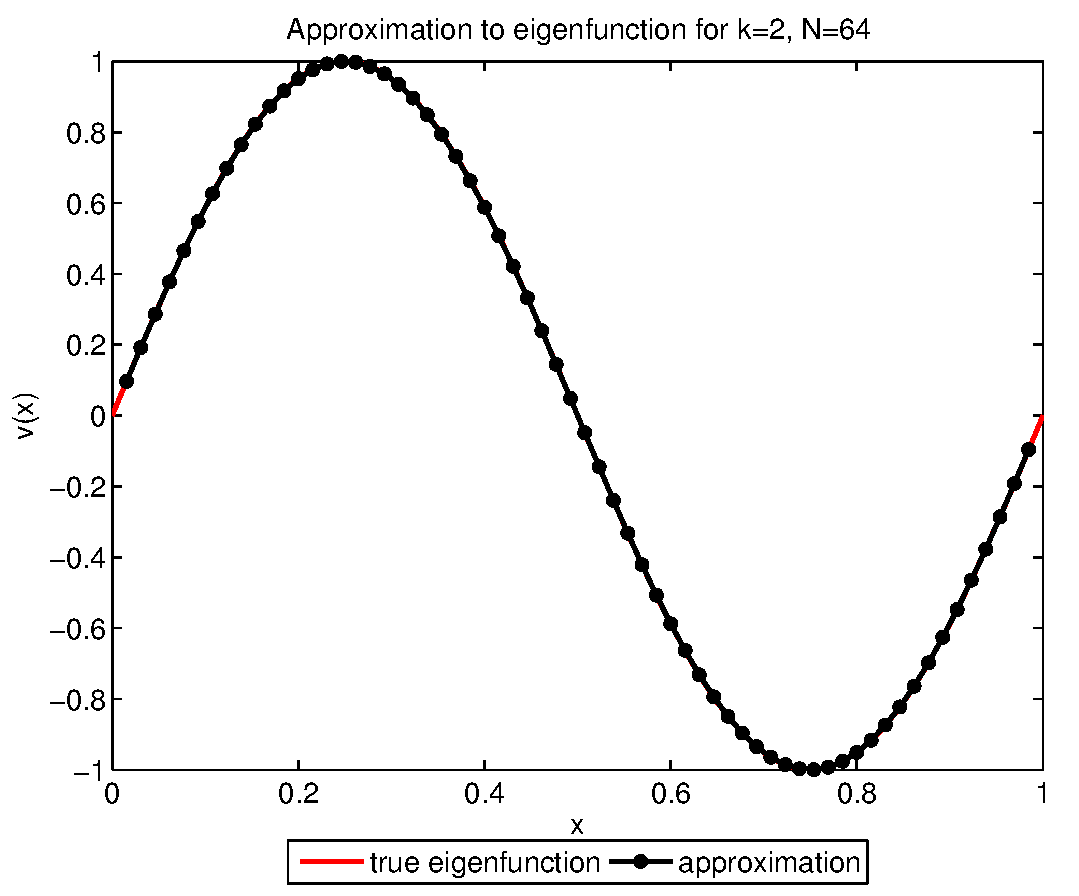
\includegraphics[scale=0.38]{lapeig_c2}

         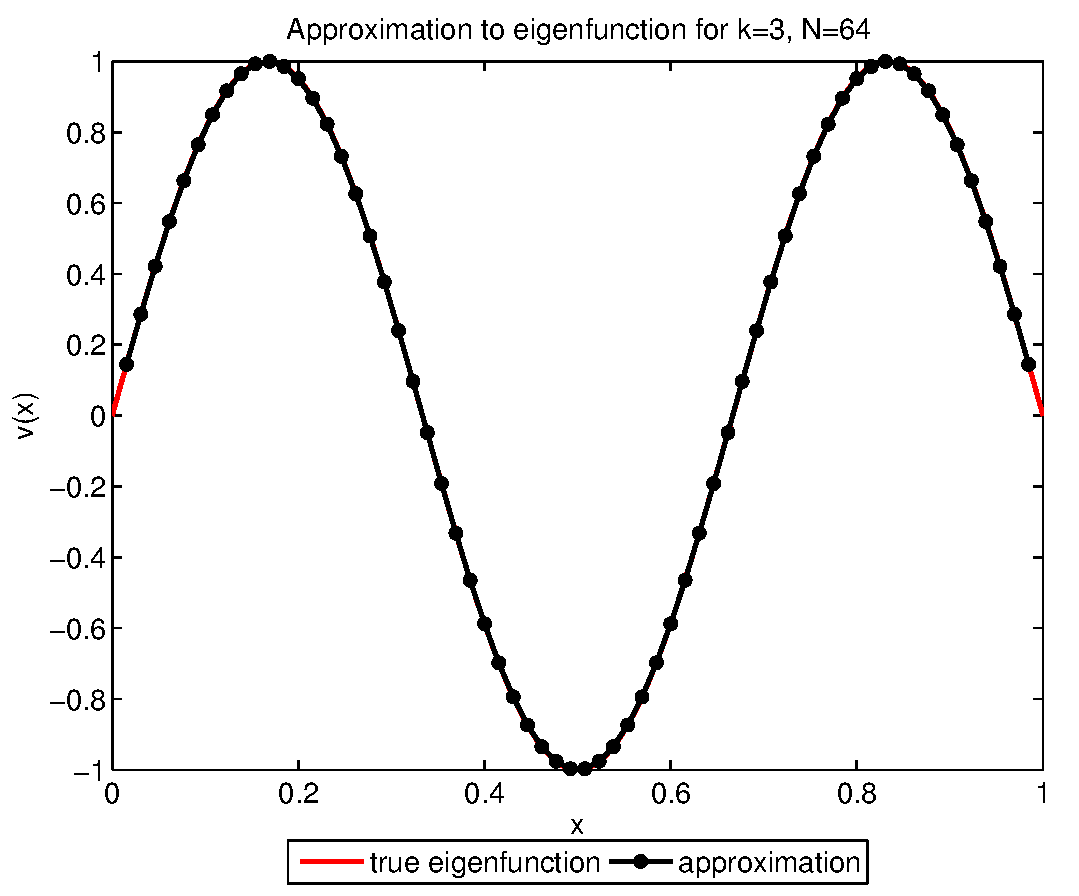
\includegraphics[scale=0.38]{lapeig_c3}\quad
         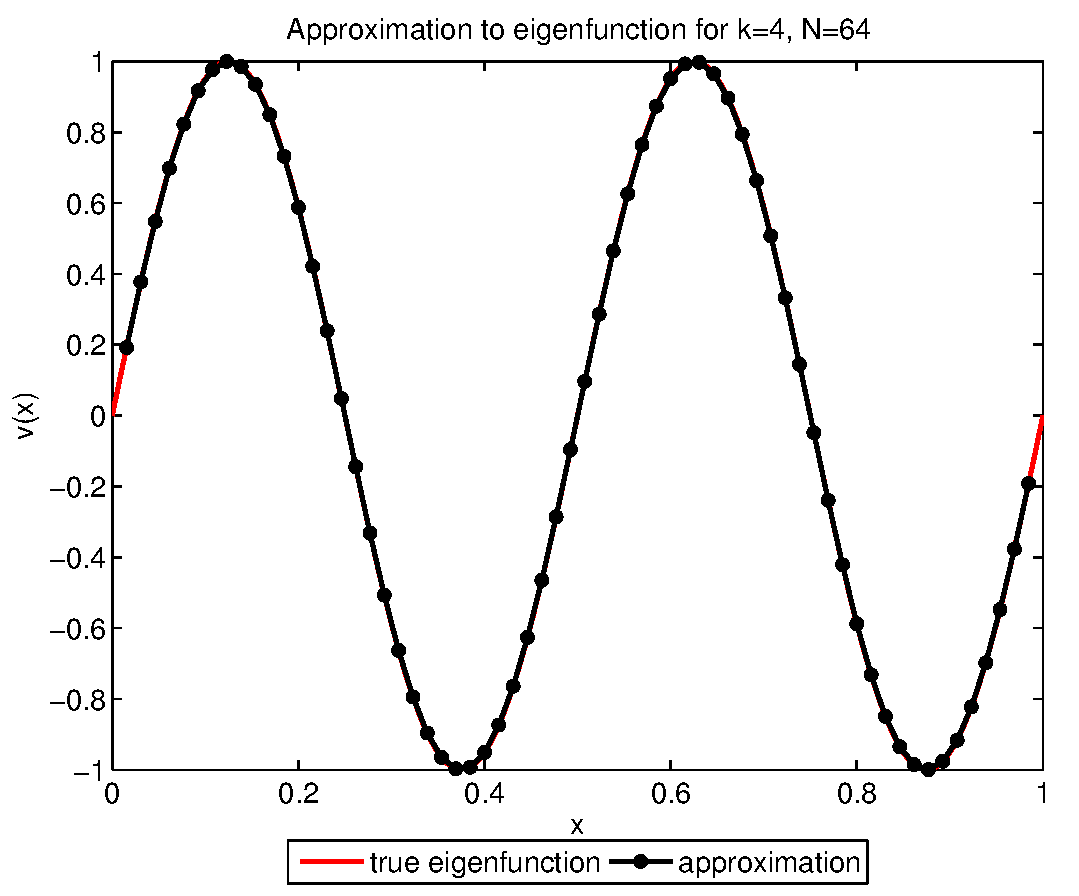
\includegraphics[scale=0.38]{lapeig_c4}

         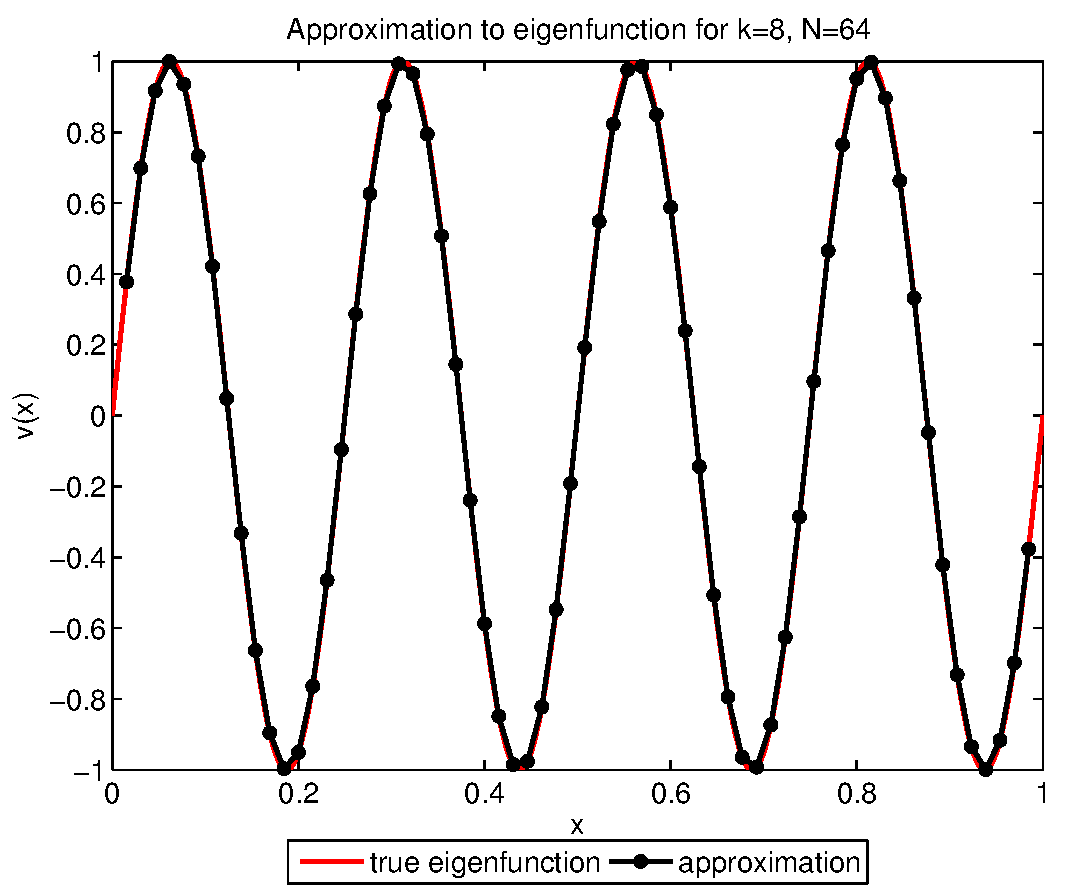
\includegraphics[scale=0.38]{lapeig_c8}\quad
         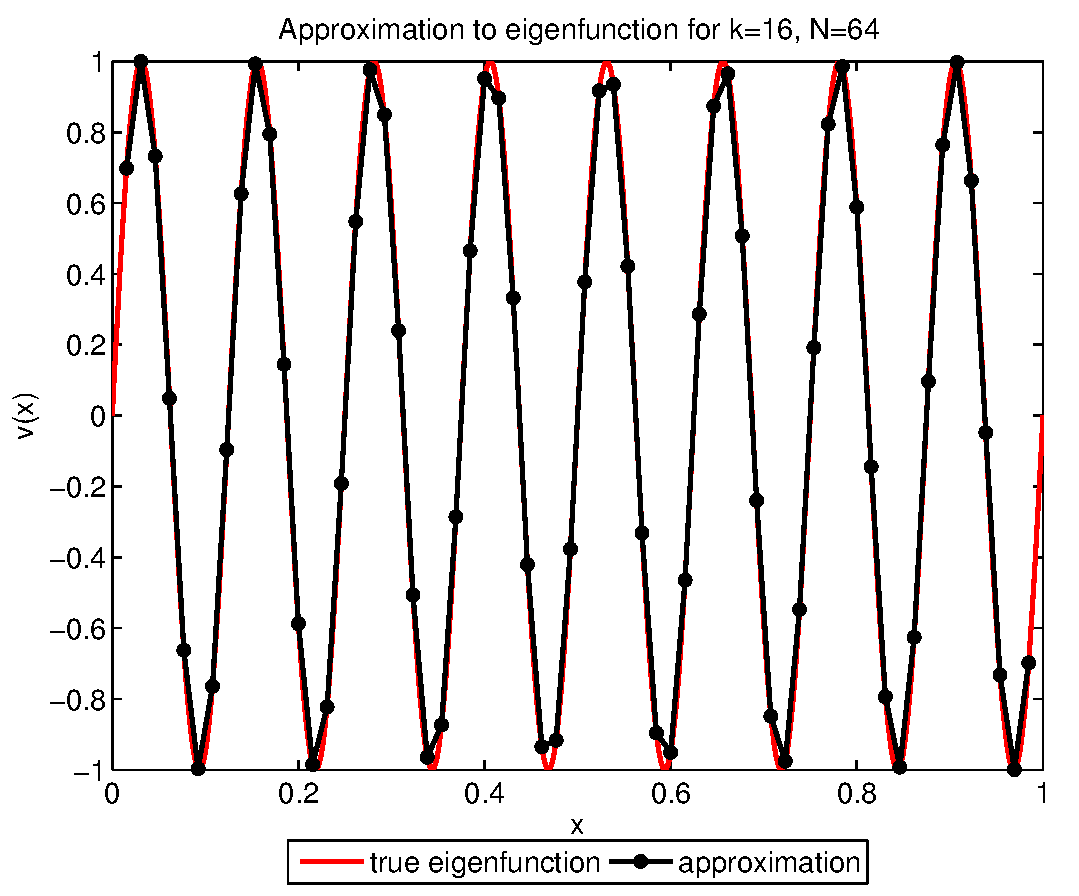
\includegraphics[scale=0.38]{lapeig_c16}

         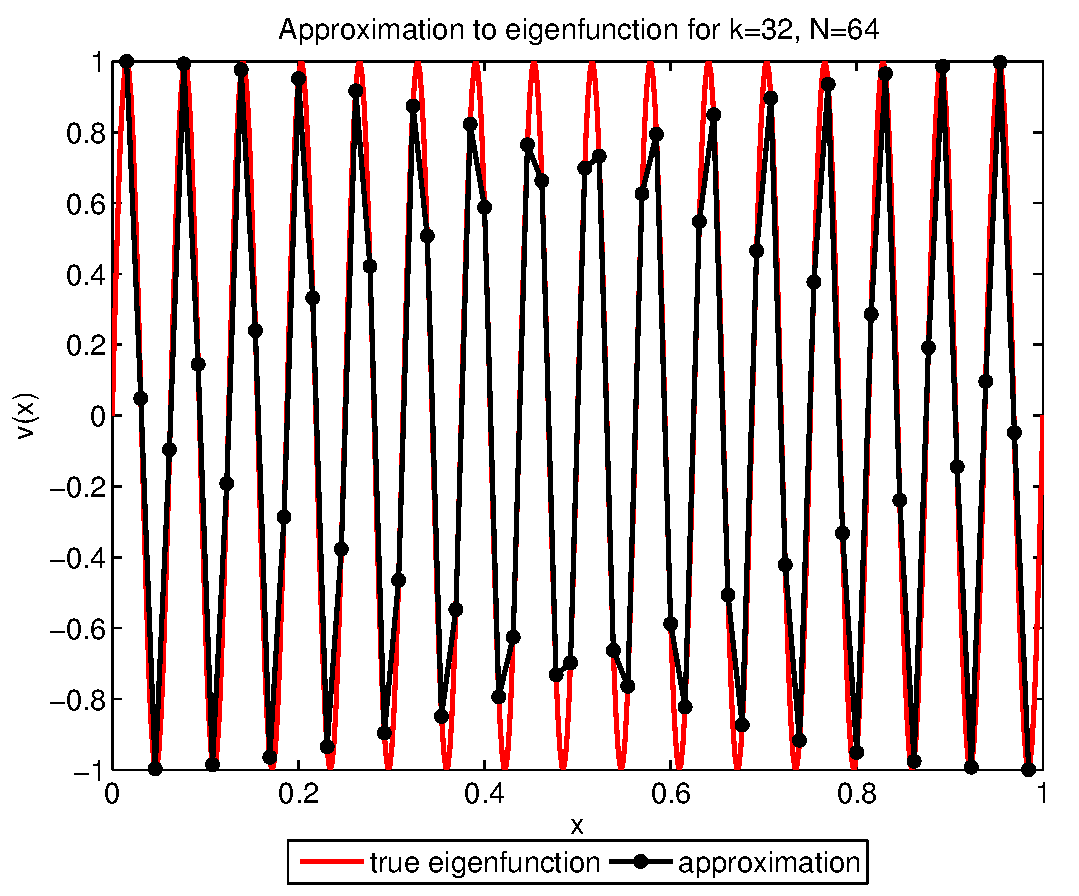
\includegraphics[scale=0.38]{lapeig_c32}\quad
         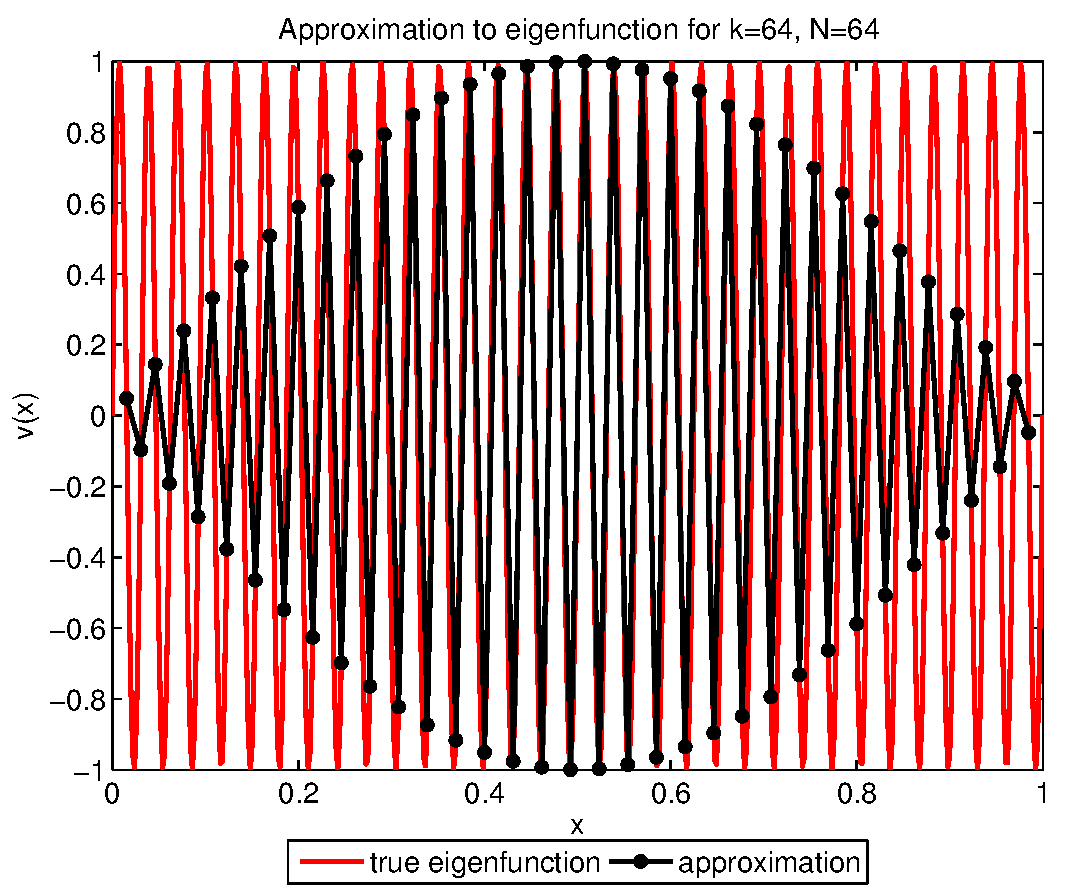
\includegraphics[scale=0.38]{lapeig_c64}
       \end{center}

\newpage
    \input  lapeigcode
\end{enumerate}
\end{solution}}{}

